\documentclass[conference]{IEEEtran}
\IEEEoverridecommandlockouts
% The preceding line is only needed to identify funding in the first footnote. If that is unneeded, please comment it out.
\usepackage{cite}
\usepackage{amsmath,amssymb,amsfonts}
\usepackage{algorithmic}
\usepackage{graphicx}
\usepackage{textcomp}
\usepackage{caption}
\usepackage{xcolor}
\usepackage{listings}
\def\BibTeX{{\rm B\kern-.05em{\sc i\kern-.025em b}\kern-.08em
    T\kern-.1667em\lower.7ex\hbox{E}\kern-.125emX}}

\lstset{language=Java}

\begin{document}

\title{Assignment 01: Distributed Sort\\
{\footnotesize Hinweis: Alle Teilnehmer haben, soweit nicht anders gekennzeichnet, zu gleichen Teilen an diesem Dokument mitgewirkt.}
\thanks{Prof. Dr. David Spieler - Big Data Analytics - Summer Term 2022}
}

\author{\IEEEauthorblockN{Lukas Johannes Foerner}
\IEEEauthorblockA{\textit{Hochschule München} \\
\textit{Fakultät 07, IF}\\
München, Deutschland \\
lukas.foerner@hm.edu}
\and
\IEEEauthorblockN{Robin Grellner}
\IEEEauthorblockA{\textit{Hochschule München} \\
\textit{Fakultät 07, IF}\\
München, Deutschland \\
robin.grellner@hm.edu}
\and
\IEEEauthorblockN{Simon Symhoven}
\IEEEauthorblockA{\textit{Hochschule München} \\
\textit{Fakultät 07, IS}\\
München, Deutschland \\
simon.symhoven@hm.edu}
}

\maketitle

\begin{abstract}
Der verwendete Quellcode ist in einem GitHub Repository verwaltet \cite{github}.
\end{abstract}

\section{Random Data}
Mit Hilfe der Methode \verb|createFiles()| werden Zufallszahlen erzeugt -- beginnend bei 10.000 Stück. Diese werden auf dem Dateisystem in Form einer Textdatei gespeichert. Jede Runde erhöhen wir die Anzahl der Datenpunkte um 10.000, solange bis die Größe von 1.000.000 Zufallszahlen erreicht ist. Die Ergebnisse der Messungen für die später verwendeten Alogrithmen werden in einer csv-Datei gespeichert. Diese zeichnet die Anzahl der Zufallszahlen, die Zeit für den Merge-Sort, sowie die Zeit für den paralellisierten Merge-Sort auf.

\section{Der Merge-Sort}
Die Methode \verb|processFiles()| startet den eigentlichen Merge-Sort. Die zuvor erzeugten Textdateien werden in einer Schleife eingelesen und jeweils die beiden Merge-Algorithmen angewendet, die Zeiten gestoppt und anschließen ein Durchschnitt über alle Runden berechnet. 
Die Methode \verb|sort()| erwartet dabei eine Liste von Zahlen und eine Anzahl der zu sortierenden Zahlen \verb|n|. Ist die \verb|n < 2|, so ist der Basisfall erreicht. Andernfalls wird die Mitte kalkuliert und zwei neue Listen erzeugt, die jeweils die Elemente \verb|0| bis \verb|n/2|, bzw. \verb|n/2| bis \verb|n| enthalten. Nun wir \verb|sort()| rekursiv auf die beiden Listen aufgerufen:

\begin{lstlisting}
public void sort(List<Integer> a, int n) {
    if (n < 2) {
        return;
    }
    int mid = n / 2;
    List<Integer> l = 
    	new ArrayList<Integer>();
    List<Integer> r = 
    	new ArrayList<Integer>();

    for (int i = 0; i < mid; i++) {
        l.add(i, a.get(i));
    }
    for (int i = mid; i < n; i++) {
        r.add(i - mid, a.get(i));
    }
    sort(l, mid);
    sort(r, n - mid);
    merge(a, l, r, mid, n - mid);
}
\end{lstlisting}

Die sortierten Teillisten werden dann wieder zusammengesetzt:

\begin{lstlisting}
public void merge(List<Integer> a, 
	List<Integer> l, List<Integer> r, 
	int left, int right) 
{
    int i = 0, j = 0, k = 0;
    while (i < left && j < right) {
        if (l.get(i) <= r.get(j)) {
            a.set(k++, l.get(i++));
        } else {
            a.set(k++, r.get(j++));
        }
    }
    while (i < left) {
        a.set(k++, l.get(i++));
    }
    while (j < right) {
        a.set(k++, r.get(j++));
    }
}
\end{lstlisting}

\section{Der parallelisierte Merge-Sort}
Das Sortieren der Teillisten kann parallelisiert werden, in dem die rekursiven Aufrufe auf \verb|sort()| in jeweils einem eigenen Thread ausgeführt werden. Sobald beide Threads beendet sind, wird \verb|merge()| aufgerufen. 
Dazu wurde die Methode \verb|sort()| angepasst:

\begin{lstlisting}
public void sortParallel(List<Integer> a, 
	int n) 
{
    // Basisfall pruefen
    // Teillisten erzeugen
    
    Thread t1 = new Thread(() -> {
	sort(l, mid);
    });
    Thread t2 = new Thread(() -> {
	sort(r, n - mid);
    });
    t1.start();
    t2.start();
    t1.join();
    t2.join();
		
    // Merge    
}
\end{lstlisting}

\section{Analyse}
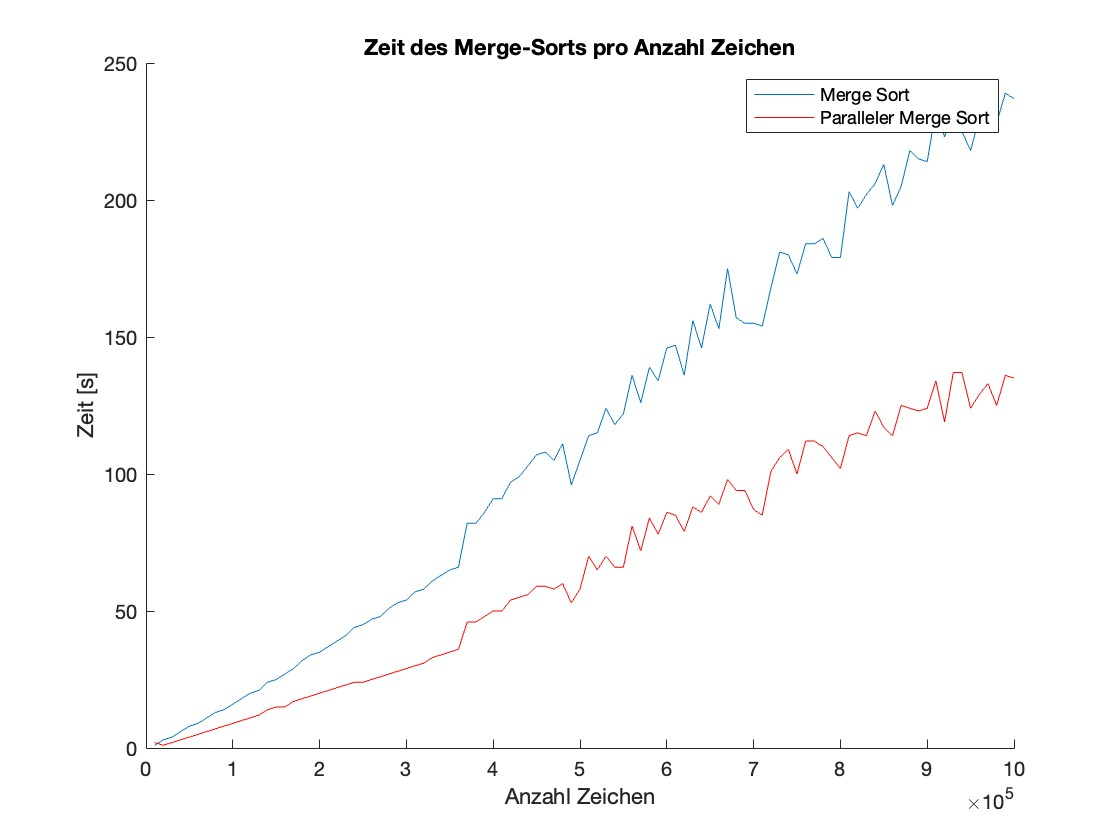
\includegraphics[width=0.5\textwidth]{figure.jpg}
Wie erwartet, hat sich die Ausführungszeit durch die Aufteilung in zwei Threads ungefähr halbiert. 
Im kleineren Bereich ($<0.2*10^5$) ist der Overhead der Threads allerdings größer als der Zeitvorteil durch die Parallelisierung.

\section{Algorithmus auf verteilten Systemen}
Können nicht alle Dateien bzw. deren Inhalte auf einem einzigen System gespeichert werden, müssen diese auf mehrere Knoten verteilt werden. Dazu muss die List der Zufallszahlen zunächst zu gleichen Teilen auf alle Knoten verteilt werden. Auf jedem dieser Knoten läuft dann der übliche Merge-Sort Algorithmus. Am Ende werden dann die vorsortierten Listen der jeweiligen Knoten im ZIp-Lock-Verfahren (Reißverschluss) zusammengefügt. Dafür wird das jeweils erste Element der jeweiligen Liste mit den anderen verglichen. Das kleinste wird auf den Speicher des ersten Knoten geschrieben, sofern Platz vorhanden ist, ansonsten auf den nächsten Knoten. Dieses Verfahren wird für jeden Index der Listen wiederholt, bis alle Elemente der Ausgangsliste sortiert und auf mehreren Knoten verteilt ist.

\begin{thebibliography}{00}
\bibitem{github} L. J. Foerner, R. Gellner, und S. Symhoven, ``simonsymhoven/big-data-hm-group-j'', GitHub, URL: https://github.com/simonsymhoven/big-data-hm-group-j, März 2022.
\end{thebibliography}

\end{document}
